\subsection{Opis języka}

Aplikacja potrafi wygenerować podstawowe elementy diagramu klas oraz diagramu przypadków użycia zdefiniowane w standardzie UML 2.0.

\subsubsection{Klasa}

Klasę definiuje się na podstawie prototypu \textbf{class}.\footnote{O prototypach będziem mowa w dalszej częsci}

\begin{lstlisting}
class Klasa
    stereotype : "Stereotyp"
    +metoda(argument) : typ
    -pole : typ = "wartosc"
    _+statyczna_metoda()
\end{lstlisting}
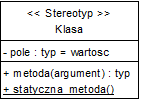
\includegraphics[width=\textwidth]{klasa}
Utworzony został obiekt o identyfikatorze \textbf{Klasa}. Na diagramie będzie to nazwą klasy. Można również nadać inną nazwę korzystając z klucza \textbf{name}(którego nie ma w przykładzie). Klucz \textbf{stereotype} pełni rolę stereotypów w języku UML. Przykładowa klasa posiada metodę(wraz ze statyczną) oraz pole. Na uwagę zasługuje okreslenie widocznosci metod i pól: +, -, ~, \#. Statyczne metody lub pola oznacza się poprzez \_.
Mając już zdefiniowaną klasę \textbf{Klasa} można utworzyć na jej podstawie następny obiekt, kopiując wszystkie ustawione wartosci kluczy z \textbf{Klasa}: \textbf{Klasa} NewObject.

\subsubsection{Relacja}

Relację okresla się na podstawie prototypu \textbf{relation}.
\begin{lstlisting}
relation
    source-object : Aktor
    source-count : 1
    source-role : "Aktor"

    target-object : uc
    target-count : *
    name : "Uzywa"

actor Aktor
usecase uc
\end{lstlisting}
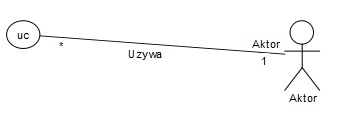
\includegraphics[width=\textwidth]{relacja}
Relację jak wyżej można zdefiniować bez nazwy, jeżeli nie ma potrzeby wykorzystywać do tworzenia nowych obiektów pochodnych od relacji. Klucz \textbf{source-object} wskazuje obiekt na diagramie od którego relacja wychodzi, natomiast \textbf{target-object} wskazuje obiekt docelowy dla końca relacji. Klucze \textbf{source-role} oraz \textbf{target-role} odpowiadają za nadanie obiektowi źródłowemu i docelowemu ról zgodnie z notacją UML. Oczywiscie nazwa relacji na diagramie poprzez \textbf{name}. Ponadto relacja może zawierać klucze: \textbf{arror} odpowiadający za okreslenie rodzaju strzałki relacji oraz \textbf{direction}, który odpowiada za miejsce umieszczenia tej strzałki.

\subsubsection{Asocjacja}

Jako przykład asocjacji można użyć powyższy listing. Oczywiscie należałoby zmienić \textbf{relation} na \textbf{association}. Oparta jest również na odpowiednim prototypie. Asocjacja ma już na wstępie zdefiniowane klucze: \textbf{arrow} i \textbf{direction}. Można traktować asocjację jako podstawową formę relacji, tzn. bez kierunków.

\subsubsection{Generalizacja}

Jest relacją o okreslonym zwrocie i kierunku strzałki.
\begin{lstlisting}
generalization
    source-object : Aktor
    target-object: Klasa

actor Aktor
class Klasa
\end{lstlisting}
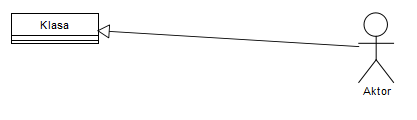
\includegraphics[width=\textwidth]{generalizacja}

\subsubsection{Agregacja}

Różni się od generalizacji typem strzałki oraz jej kierunkiem.
\begin{lstlisting}
aggregation
    source-object : Klasa
    target-object: InnaKlasa

class InnaKlasa
class Klasa
\end{lstlisting}
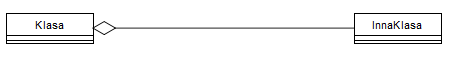
\includegraphics[width=\textwidth]{agregacja}

\subsubsection{Kompozycja}

Kompozycja różni się od generalizacji i agregacji typem strzałki oraz ma kierunek zdefiniowany taki jak agregacja.
\begin{lstlisting}
composition 
    source-object : Aktor
    target-object : Notatka
    
actor Aktor
note Notatka
\end{lstlisting}
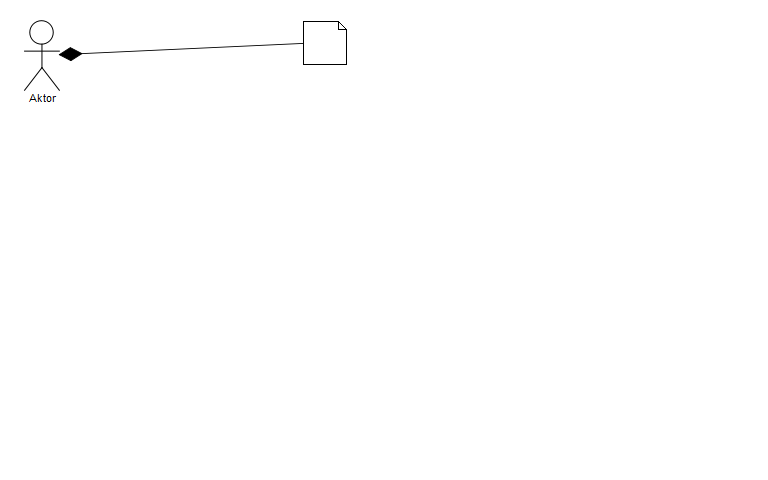
\includegraphics[width=\textwidth]{kompozycja}

\subsubsection{Notatka}

Notatka może posiadać tylko tekst. Nie ma zdefiniowanych innych kluczy oprócz \textbf{text}.
\begin{lstlisting}
note 
    text : "Notatka Notatka Notatka Notatka Notatka Notatka Notatka Notatka"
\end{lstlisting}
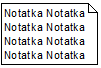
\includegraphics[width=\textwidth]{notatka}

\subsubsection{Aktor i przypadek użycia}

Aktor posiada tylko klucz \textbf{name}. Podobnie przypadek użycia.
\begin{lstlisting}
actor Aktor

usecase uc
    name : "Przypadek uzycia"
\end{lstlisting}
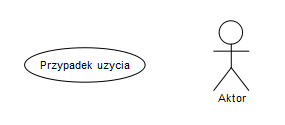
\includegraphics[width=\textwidth]{aktor_uc}